\documentclass[11pt,a4paper]{article}
\usepackage[utf8]{inputenc}
\usepackage[T1]{fontenc}
\usepackage[spanish,es-noshorthands]{babel}
\usepackage[margin=2.2cm]{geometry}
\usepackage{graphicx,float,longtable,array,booktabs,hyperref}
\graphicspath{{evidencias/}}
\hypersetup{colorlinks=true,linkcolor=black,urlcolor=blue}
% Para continuar la numeración del TP I: ajustar el número de la última sección del TP I
\setcounter{section}{7}

\title{Proyecto Integrador II -- De Monolito a Cloud Native: BookStack\\[4pt]\large Arquitectura Web -- FP-UNA -- Fases 5, 6 y 7}
\author{Samir Galeano \and Fernando Servián \and Jazmín Figueredo}
\date{15 de noviembre de 2026}

\begin{document}
\maketitle
\noindent Repositorio: \url{https://github.com/samir-galeano/Trabajo-Pr-ctico-Integrador-II---Arquitectura-Web} (etiqueta \texttt{v2.0.0}).

Este informe continúa el del TP Integrador I. Documenta la descomposición del monolito BookStack en microservicios (Fase 5), su construcción, contenerización y despliegue distribuido (Fase 6) y su operación cloud native: resiliencia, escalabilidad, observabilidad y seguridad (Fase 7). Las evidencias siguen la numeración F5-E1 a F7-E14 y la matriz de pruebas continúa la Tabla 5 del TP I desde P26.

\tableofcontents
\newpage

%=====================================================================
\section{Fase 5: diseño y descomposición del monolito}
%=====================================================================
\subsection{Análisis del monolito y contextos delimitados}
Se inventariaron las tablas de BookStack por módulo consultando \texttt{information\_schema} (F5-E1) y se construyó la matriz de acoplamiento módulo $\times$ tabla, incluidas las relaciones polimórficas (F5-E2). A partir de ese análisis se definió el mapa de contextos (F5-E3) y se eligieron los cuatro servicios a extraer:
\begin{itemize}
  \item \textbf{S1 search-svc}: búsqueda de texto completo con índice propio en PostgreSQL, reindexado por eventos.
  \item \textbf{S2 audit-svc}: registro de auditoría de las ediciones, consultable por entidad y rango de fechas.
  \item \textbf{S3 export-svc}: exportación asíncrona de páginas y libros a PDF o Markdown, almacenada en MinIO.
  \item \textbf{S4 media-svc}: subida de imágenes y generación de miniaturas.
\end{itemize}

\subsection{Decisiones de arquitectura (ADR-006 a ADR-011)}
\begin{description}
  \item[ADR-006 -- Strangler Fig.] Extracción incremental de funcionalidades. La integración con BookStack es exclusivamente por API REST, webhooks y un API Gateway; no se modifica su código fuente.
  \item[ADR-007 -- Broker.] NATS JetStream: persistencia, streams, consumidores durables y confirmación de entrega, con un sobre de evento común (\texttt{event\_id}, \texttt{type}, \texttt{occurred\_at}, \texttt{request\_id}, \texttt{payload}).
  \item[ADR-008 -- Orquestación.] Docker Compose en un nodo. \emph{Reemplazado por ADR-011}; Compose se mantiene para desarrollo.
  \item[ADR-009 -- Base de datos por servicio.] Cada servicio administra sus datos (Database per Service); ningún servicio accede a las tablas de BookStack.
  \item[ADR-010 -- Consistencia eventual.] Idempotencia por \texttt{event\_id}, reintentos limitados y cola de mensajes fallidos (DLQ).
  \item[ADR-011 -- Docker Swarm en dos nodos.] Necesario para escalar \texttt{export-worker} entre nodos, autorrecuperación real ante caídas, secretos cifrados del clúster y actualizaciones rodantes sin corte.
\end{description}

\subsection{Contratos y diagramas}
Los contratos OpenAPI de los cuatro servicios y el contrato AsyncAPI de los eventos se validaron sin errores (F5-E4). Los diagramas C4 de contexto y de contenedores (F5-E5, F5-E6) y los diagramas de secuencia con caminos de error (F5-E7) están en \texttt{cna/docs/diagramas/}. El plan de migración y riesgos está en \texttt{cna/docs/plan\_migracion\_riesgos.md}.

\subsection{Evidencias de la Fase 5}
\subsubsection*{F5-E1 (P26) -- Tablas por módulo vía information\_schema}
\begin{figure}[H]
\centering
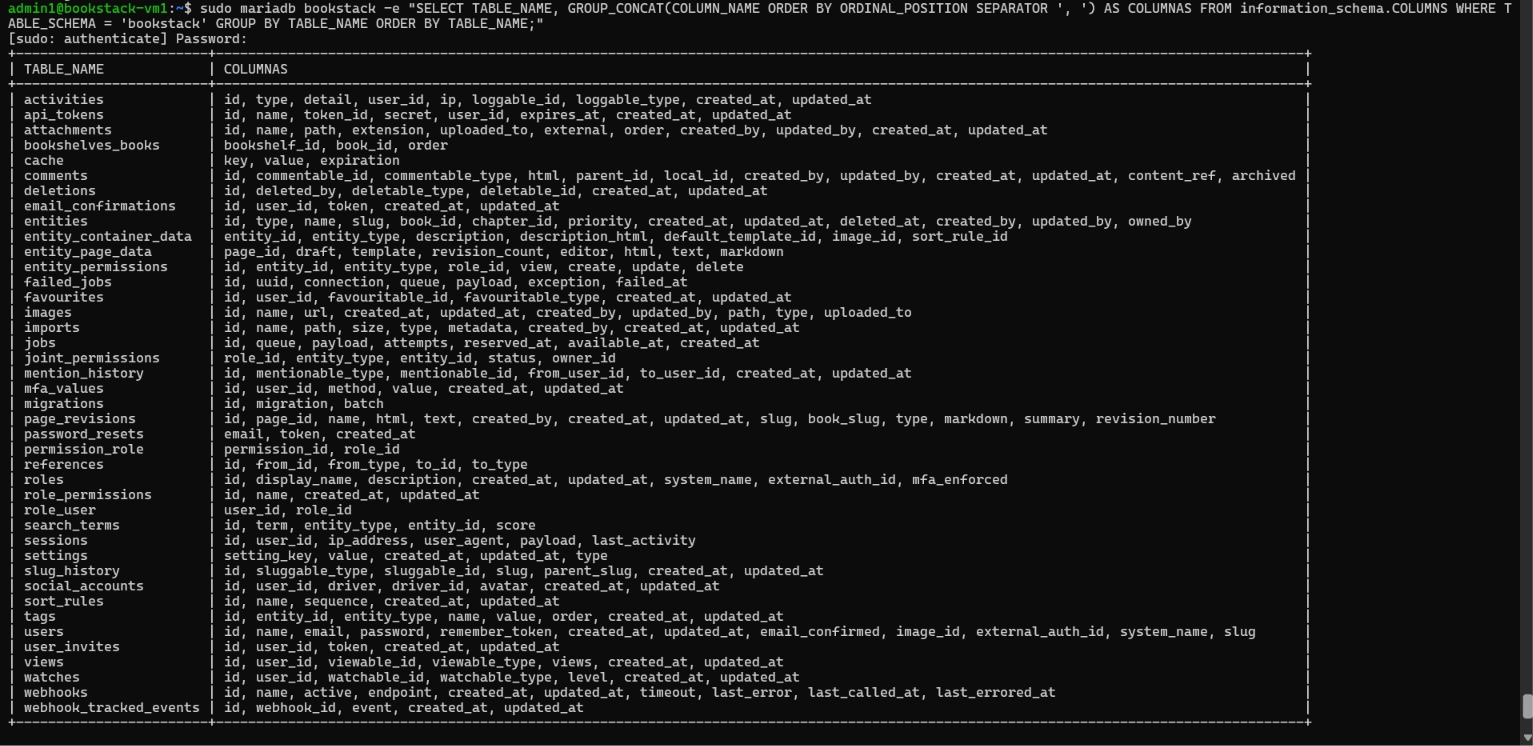
\includegraphics[width=0.9\linewidth,height=0.42\textheight,keepaspectratio]{F5-E1_inventario_tablas.png}
\caption{F5-E1: Tablas por módulo vía information\_schema}
\label{fig:F5-E1-1}
\end{figure}
\subsubsection*{F5-E2 (P27) -- Matriz de acoplamiento módulo × tabla}
\begin{figure}[H]
\centering
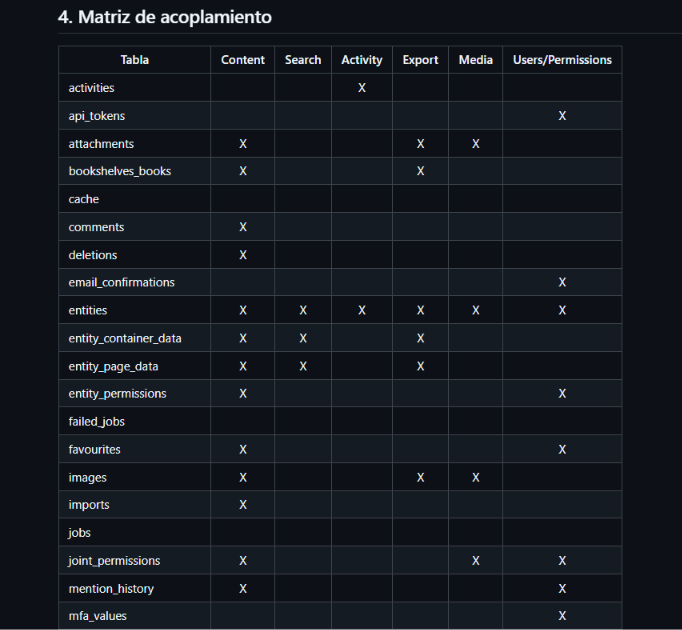
\includegraphics[width=0.9\linewidth,height=0.42\textheight,keepaspectratio]{F5-E2_matriz_parte1.png}
\caption{F5-E2: Matriz de acoplamiento módulo × tabla (parte 1)}
\label{fig:F5-E2-1}
\end{figure}
\begin{figure}[H]
\centering
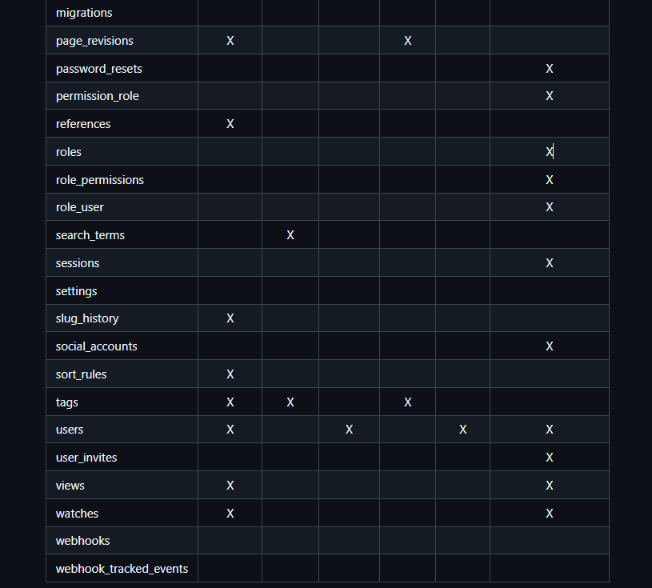
\includegraphics[width=0.9\linewidth,height=0.42\textheight,keepaspectratio]{F5-E2_matriz_parte2.png}
\caption{F5-E2: Matriz de acoplamiento módulo × tabla (parte 2)}
\label{fig:F5-E2-2}
\end{figure}
\begin{figure}[H]
\centering
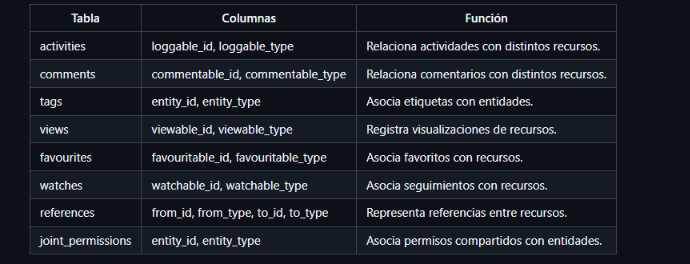
\includegraphics[width=0.9\linewidth,height=0.42\textheight,keepaspectratio]{F5-E2_relaciones_polimorficas.png}
\caption{F5-E2: Matriz de acoplamiento módulo × tabla (parte 3)}
\label{fig:F5-E2-3}
\end{figure}
\subsubsection*{F5-E3 (P28) -- Mapa de contextos (DDD)}
\begin{figure}[H]
\centering
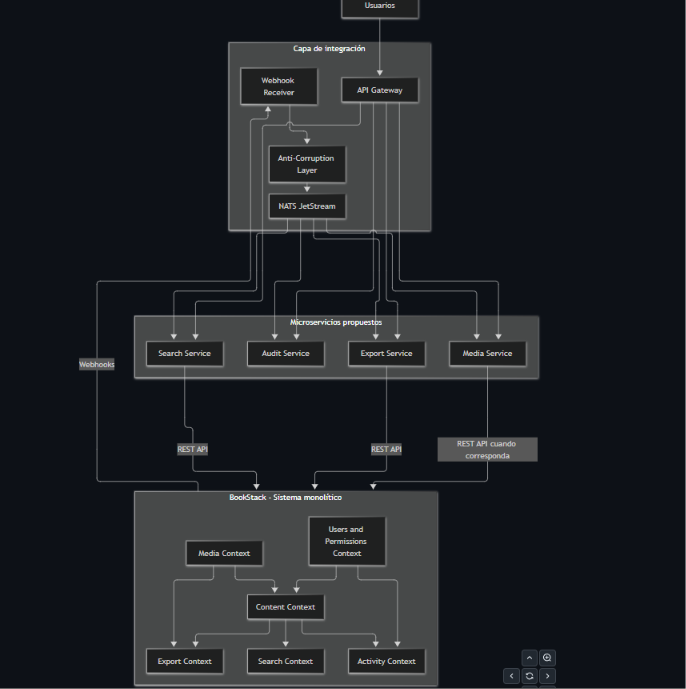
\includegraphics[width=0.9\linewidth,height=0.42\textheight,keepaspectratio]{F5-E3_mapa_contextos_ddd.png}
\caption{F5-E3: Mapa de contextos (DDD)}
\label{fig:F5-E3-1}
\end{figure}
\subsubsection*{F5-E4 (P29) -- Contratos OpenAPI/AsyncAPI validados}
\begin{figure}[H]
\centering
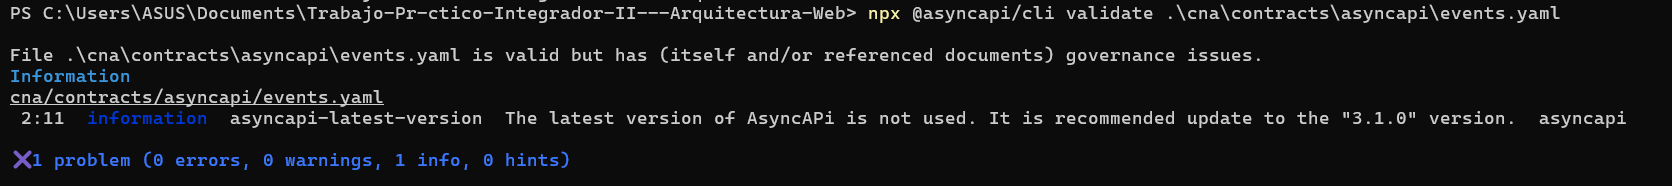
\includegraphics[width=0.9\linewidth,height=0.42\textheight,keepaspectratio]{F5-E4_validacion_asyncapi.png}
\caption{F5-E4: Contratos OpenAPI/AsyncAPI validados (parte 1)}
\label{fig:F5-E4-1}
\end{figure}
\begin{figure}[H]
\centering
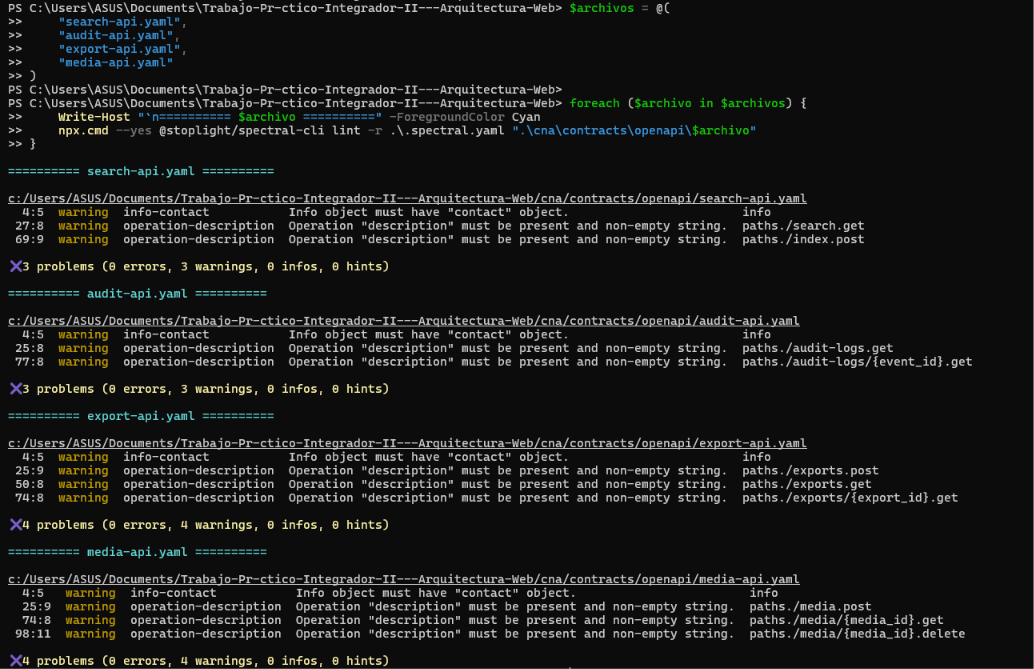
\includegraphics[width=0.9\linewidth,height=0.42\textheight,keepaspectratio]{F5-E4_validacion_openapi.png}
\caption{F5-E4: Contratos OpenAPI/AsyncAPI validados (parte 2)}
\label{fig:F5-E4-2}
\end{figure}
\subsubsection*{F5-E5 (P30) -- Diagrama C4 nivel 1 (contexto)}
\begin{figure}[H]
\centering
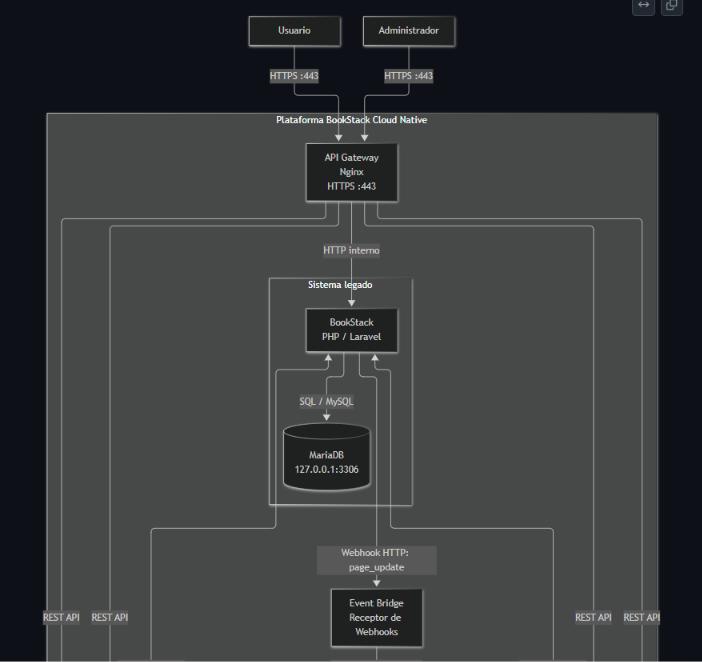
\includegraphics[width=0.9\linewidth,height=0.42\textheight,keepaspectratio]{F5-E5_c4_contexto_parte1.png}
\caption{F5-E5: Diagrama C4 nivel 1 (contexto) (parte 1)}
\label{fig:F5-E5-1}
\end{figure}
\begin{figure}[H]
\centering
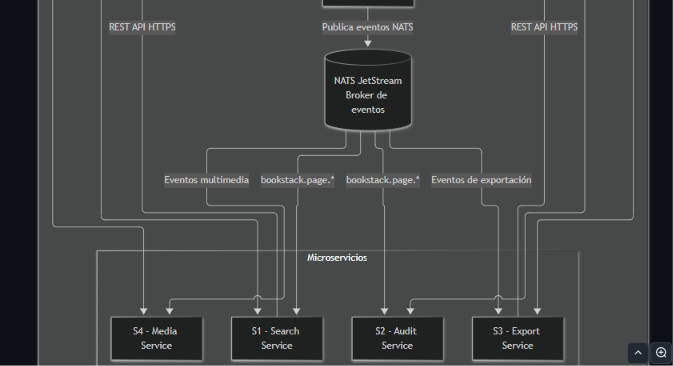
\includegraphics[width=0.9\linewidth,height=0.42\textheight,keepaspectratio]{F5-E5_c4_contexto_parte2.png}
\caption{F5-E5: Diagrama C4 nivel 1 (contexto) (parte 2)}
\label{fig:F5-E5-2}
\end{figure}
\subsubsection*{F5-E6 (P31) -- Diagrama C4 nivel 2 (contenedores)}
\begin{figure}[H]
\centering
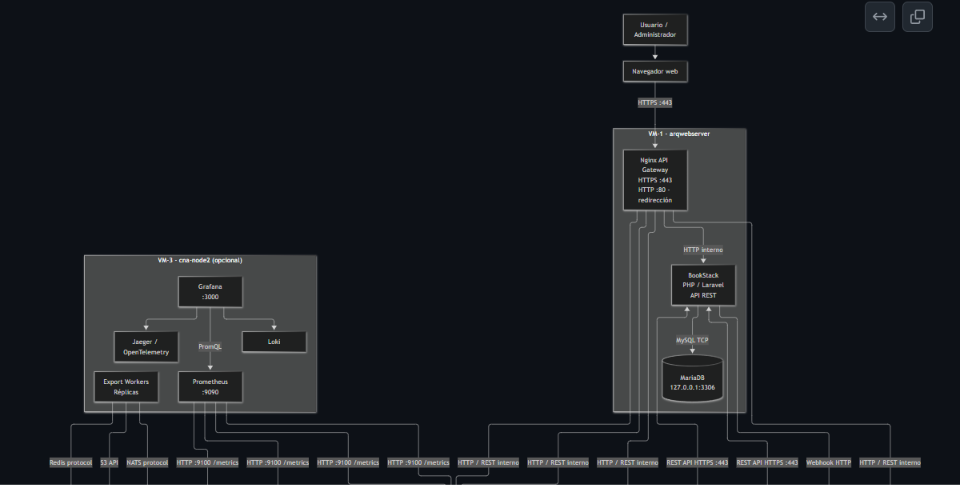
\includegraphics[width=0.9\linewidth,height=0.42\textheight,keepaspectratio]{F5-E6_c4_contenedores_parte1.png}
\caption{F5-E6: Diagrama C4 nivel 2 (contenedores) (parte 1)}
\label{fig:F5-E6-1}
\end{figure}
\begin{figure}[H]
\centering
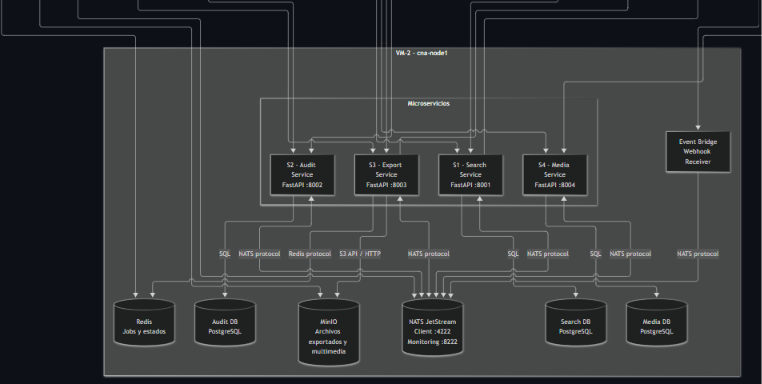
\includegraphics[width=0.9\linewidth,height=0.42\textheight,keepaspectratio]{F5-E6_c4_contenedores_parte2.png}
\caption{F5-E6: Diagrama C4 nivel 2 (contenedores) (parte 2)}
\label{fig:F5-E6-2}
\end{figure}
\subsubsection*{F5-E7 (P32) -- Diagramas de secuencia con caminos de error}
\begin{figure}[H]
\centering
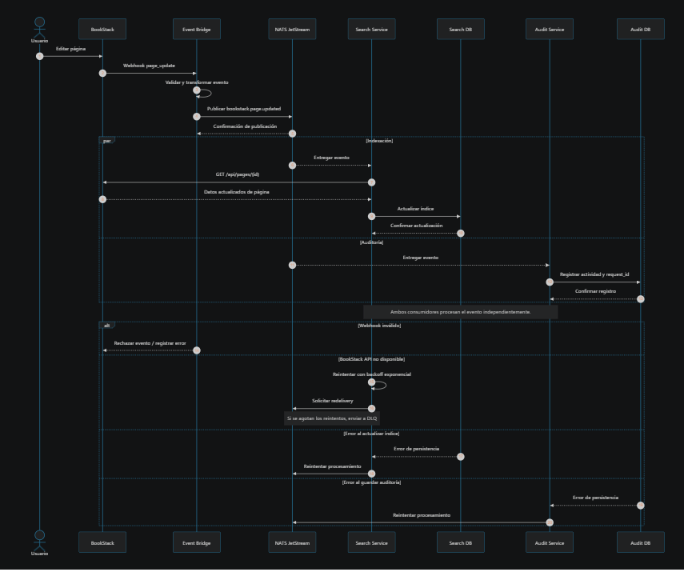
\includegraphics[width=0.9\linewidth,height=0.42\textheight,keepaspectratio]{F5-E7_secuencia_1.png}
\caption{F5-E7: Diagramas de secuencia con caminos de error (parte 1)}
\label{fig:F5-E7-1}
\end{figure}
\begin{figure}[H]
\centering
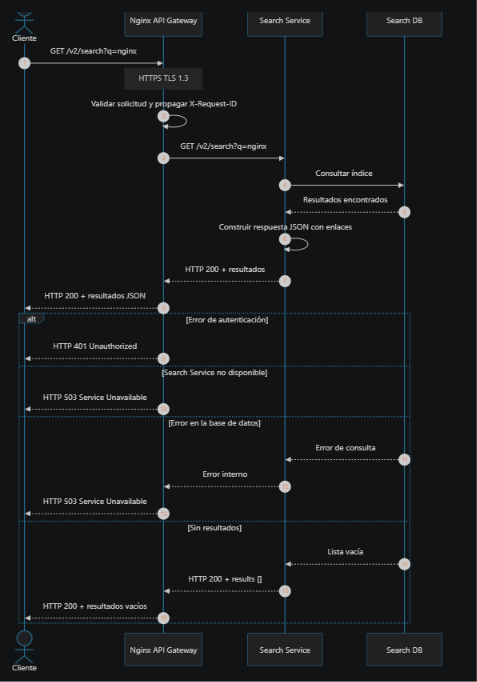
\includegraphics[width=0.9\linewidth,height=0.42\textheight,keepaspectratio]{F5-E7_secuencia_2.png}
\caption{F5-E7: Diagramas de secuencia con caminos de error (parte 2)}
\label{fig:F5-E7-2}
\end{figure}
\begin{figure}[H]
\centering
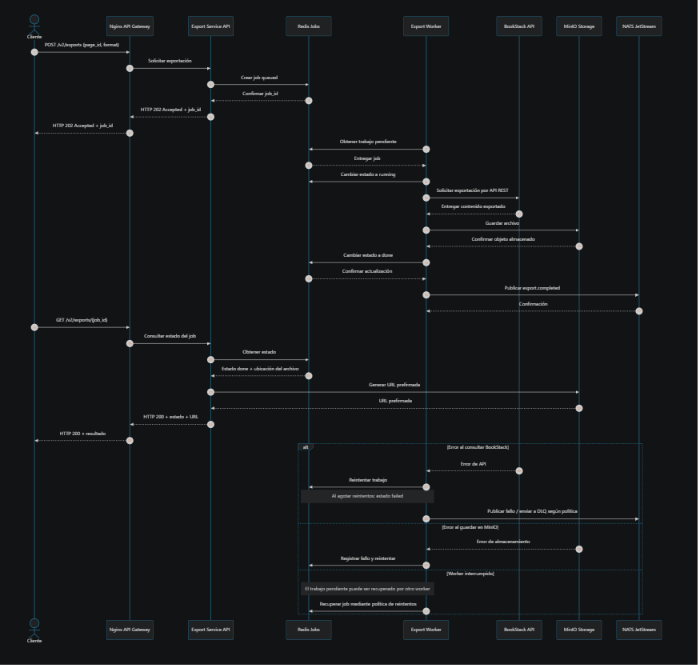
\includegraphics[width=0.9\linewidth,height=0.42\textheight,keepaspectratio]{F5-E7_secuencia_3.png}
\caption{F5-E7: Diagramas de secuencia con caminos de error (parte 3)}
\label{fig:F5-E7-3}
\end{figure}

\newpage
%=====================================================================
\section{Fase 6: construcción, contenerización y despliegue distribuido}
%=====================================================================
\subsection{Infraestructura}
VM-1 aloja el monolito BookStack y el gateway Nginx (\texttt{api.bookstack.local}, TLS con certificado de doble SAN, F6-E3); VM-2 ejecuta los microservicios, el broker, los almacenes y la observabilidad. El firewall de cada nodo (F6-E2) solo expone 22 y 443 en VM-1; los puertos publicados por Docker se filtran en la cadena \texttt{DOCKER-USER} (hallazgo H-07).

\subsection{Microservicios}
\begin{itemize}
  \item \textbf{search-svc}: indexación inicial por la API paginada y reindexación al recibir eventos; búsqueda con resaltado y enlace (F6-E4).
  \item \textbf{audit-svc}: consumidor durable con PostgreSQL propio; \texttt{event\_id} como clave primaria garantiza la idempotencia (F6-E5).
  \item \textbf{export-svc + export-worker}: el API encola en Redis y responde 202; los workers, separados del API, exportan y suben a MinIO; estados \texttt{queued}, \texttt{running}, \texttt{done}, \texttt{failed} (F6-E6, F6-E7).
  \item \textbf{media-svc}: subida de imágenes, miniaturas y evento \texttt{media.uploaded} (F6-E8).
\end{itemize}

\subsection{Contenerización}
Imágenes multi-etapa sobre \texttt{python:3.12-slim}, usuario no root (UID 10001), límites de CPU y memoria, healthcheck y sistema de archivos de solo lectura (F6-E9, F6-E10). En Swarm las imágenes se etiquetan \texttt{<versión>-<commit>} (H-08).

\subsection{Integración y broker}
BookStack envía webhooks (F6-E11) a event-bridge, que valida el token y publica en el stream \texttt{BOOKSTACK} de JetStream (F6-E12). Tras cinco intentos fallidos el mensaje pasa a la DLQ (F6-E13). El usuario de servicio de BookStack tiene un rol de solo lectura con acceso a la API.

\subsection{Gateway y despliegue}
El gateway Nginx enruta \texttt{/v2/*} a cada servicio con TLS, rate limiting (429, F6-E15) y respuesta 503 JSON ante caídas (F6-E14). Todo el sistema se despliega con un comando desde un repositorio limpio: \texttt{./cna/deploy/setup-env.sh} y \texttt{docker compose up -d} (CA-7), o \texttt{./cna/deploy/swarm/deploy.sh} en Swarm (F6-E16).

\subsection{Evidencias de la Fase 6}
\subsubsection*{F6-E1 (P33) -- Nodos activos del motor Docker}
\begin{figure}[H]
\centering
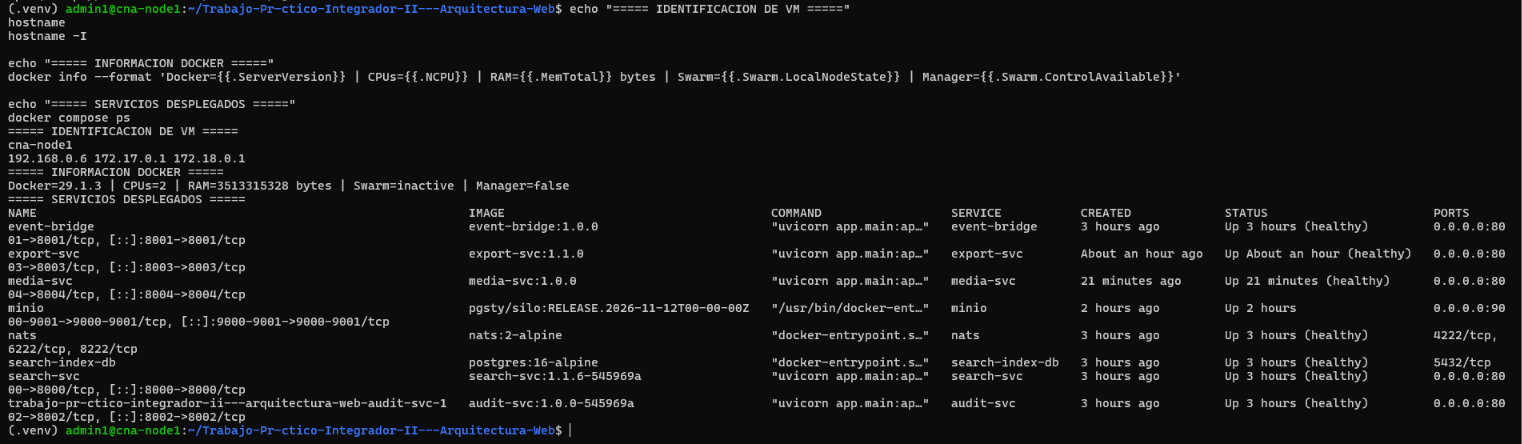
\includegraphics[width=0.9\linewidth,height=0.42\textheight,keepaspectratio]{F6-E1_01_docker_info_nodos.png}
\caption{F6-E1: Nodos activos del motor Docker}
\label{fig:F6-E1-1}
\end{figure}
\subsubsection*{F6-E2 (P34) -- ufw status verbose de cada nodo}
\begin{figure}[H]
\centering
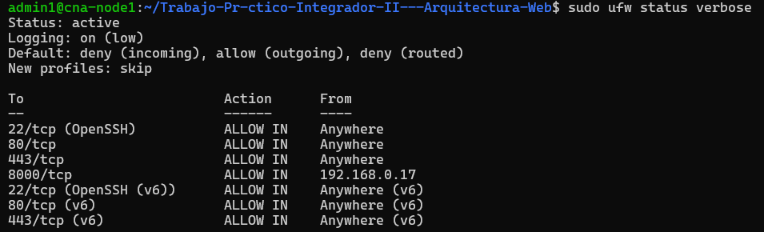
\includegraphics[width=0.9\linewidth,height=0.42\textheight,keepaspectratio]{F6-E2_01_firewall_vm2.png}
\caption{F6-E2: ufw status verbose de cada nodo}
\label{fig:F6-E2-1}
\end{figure}
\subsubsection*{F6-E3 (P35) -- Certificado X.509 con doble SAN}
\begin{figure}[H]
\centering
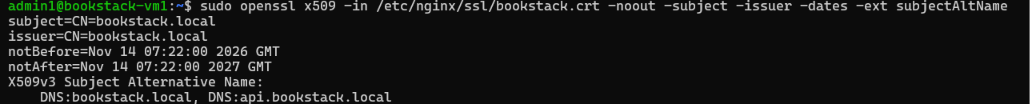
\includegraphics[width=0.9\linewidth,height=0.42\textheight,keepaspectratio]{F6-E3_01_certificado_SAN.png}
\caption{F6-E3: Certificado X.509 con doble SAN}
\label{fig:F6-E3-1}
\end{figure}
\subsubsection*{F6-E4 (P36) -- Búsqueda vía gateway antes/después de editar}
\begin{figure}[H]
\centering
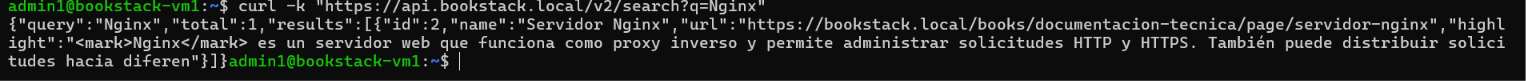
\includegraphics[width=0.9\linewidth,height=0.42\textheight,keepaspectratio]{F6-E4_01_busqueda_antes_edicion.png}
\caption{F6-E4: Búsqueda vía gateway antes/después de editar (parte 1)}
\label{fig:F6-E4-1}
\end{figure}
\begin{figure}[H]
\centering
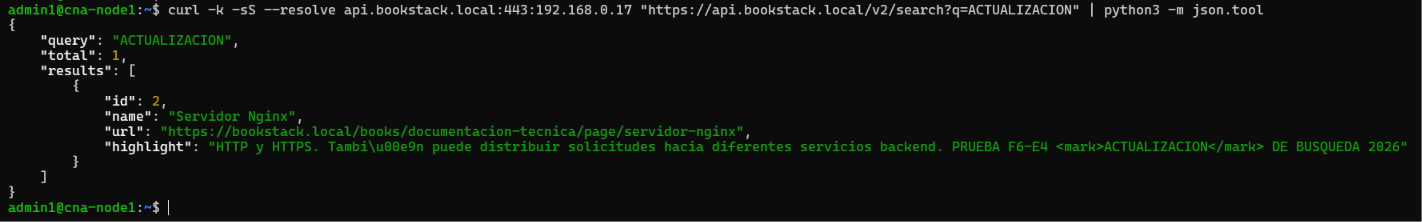
\includegraphics[width=0.9\linewidth,height=0.42\textheight,keepaspectratio]{F6-E4_02_busqueda_despues_edicion.png}
\caption{F6-E4: Búsqueda vía gateway antes/después de editar (parte 2)}
\label{fig:F6-E4-2}
\end{figure}
\begin{figure}[H]
\centering
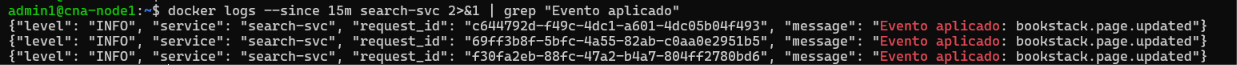
\includegraphics[width=0.9\linewidth,height=0.42\textheight,keepaspectratio]{F6-E4_03_evento_procesado_search.png}
\caption{F6-E4: Búsqueda vía gateway antes/después de editar (parte 3)}
\label{fig:F6-E4-3}
\end{figure}
\begin{figure}[H]
\centering
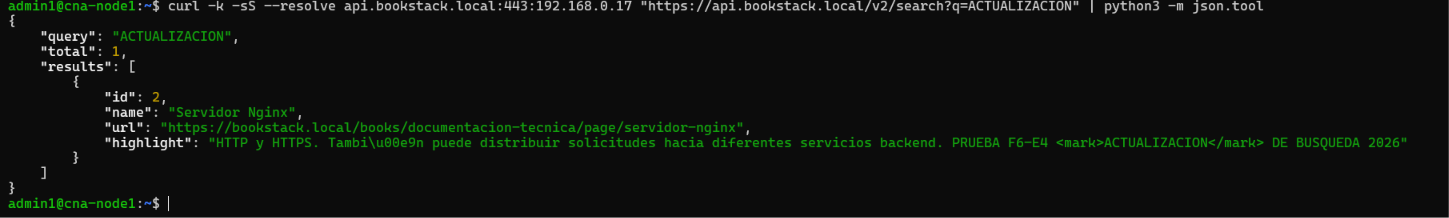
\includegraphics[width=0.9\linewidth,height=0.42\textheight,keepaspectratio]{F6-E4_04_resultado_search.png}
\caption{F6-E4: Búsqueda vía gateway antes/después de editar (parte 4)}
\label{fig:F6-E4-4}
\end{figure}
\subsubsection*{F6-E5 (P37) -- Idempotencia ante evento duplicado}
\begin{figure}[H]
\centering
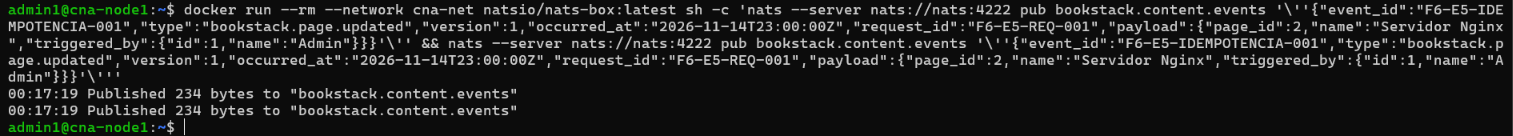
\includegraphics[width=0.9\linewidth,height=0.42\textheight,keepaspectratio]{F6-E5_01_evento_publicado_dos_veces.png}
\caption{F6-E5: Idempotencia ante evento duplicado (parte 1)}
\label{fig:F6-E5-1}
\end{figure}
\begin{figure}[H]
\centering
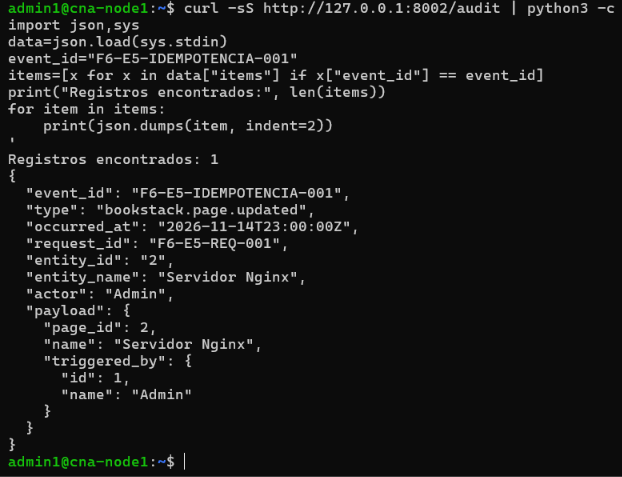
\includegraphics[width=0.9\linewidth,height=0.42\textheight,keepaspectratio]{F6-E5_02_un_solo_registro_audit.png}
\caption{F6-E5: Idempotencia ante evento duplicado (parte 2)}
\label{fig:F6-E5-2}
\end{figure}
\subsubsection*{F6-E6 (P38) -- Ciclo completo de un job de exportación}
\begin{figure}[H]
\centering
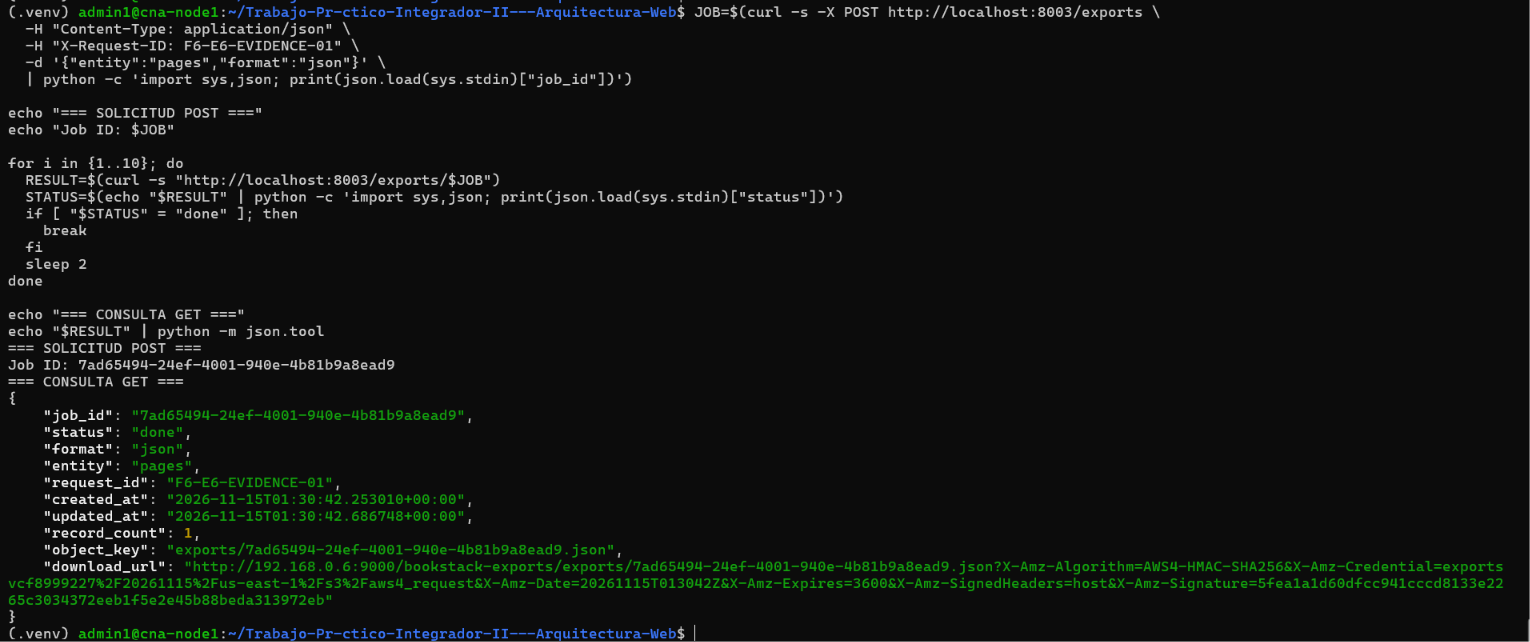
\includegraphics[width=0.9\linewidth,height=0.42\textheight,keepaspectratio]{F6-E6_01_ciclo_exportacion_completo.png}
\caption{F6-E6: Ciclo completo de un job de exportación (parte 1)}
\label{fig:F6-E6-1}
\end{figure}
\begin{figure}[H]
\centering
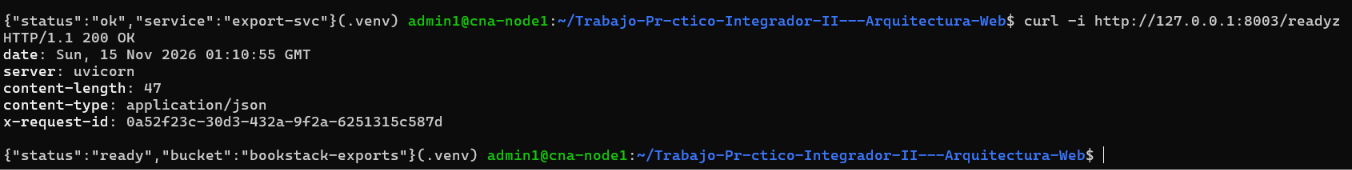
\includegraphics[width=0.9\linewidth,height=0.42\textheight,keepaspectratio]{F6-E6_02_export_svc_ready_minio.png}
\caption{F6-E6: Ciclo completo de un job de exportación (parte 2)}
\label{fig:F6-E6-2}
\end{figure}
\begin{figure}[H]
\centering
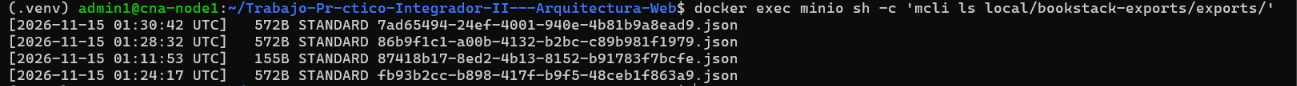
\includegraphics[width=0.9\linewidth,height=0.42\textheight,keepaspectratio]{F6-E6_02_objeto_en_minio.png}
\caption{F6-E6: Ciclo completo de un job de exportación (parte 3)}
\label{fig:F6-E6-3}
\end{figure}
\begin{figure}[H]
\centering
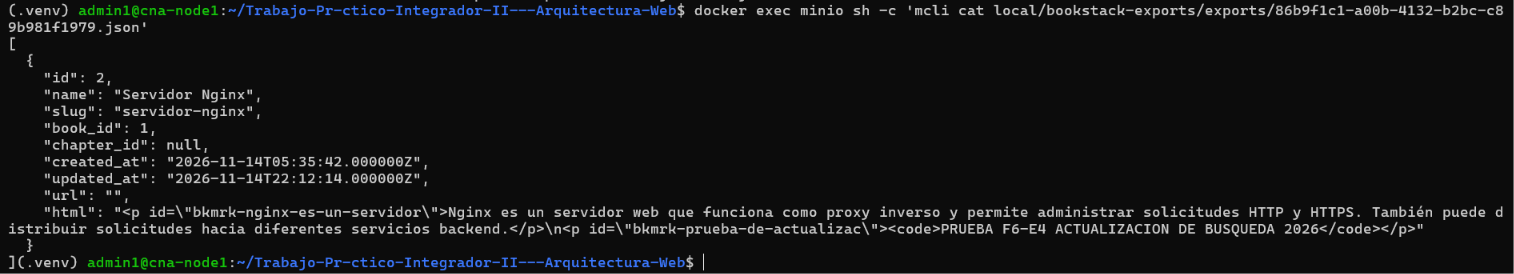
\includegraphics[width=0.9\linewidth,height=0.42\textheight,keepaspectratio]{F6-E6_03_contenido_exportado.png}
\caption{F6-E6: Ciclo completo de un job de exportación (parte 4)}
\label{fig:F6-E6-4}
\end{figure}
\begin{figure}[H]
\centering
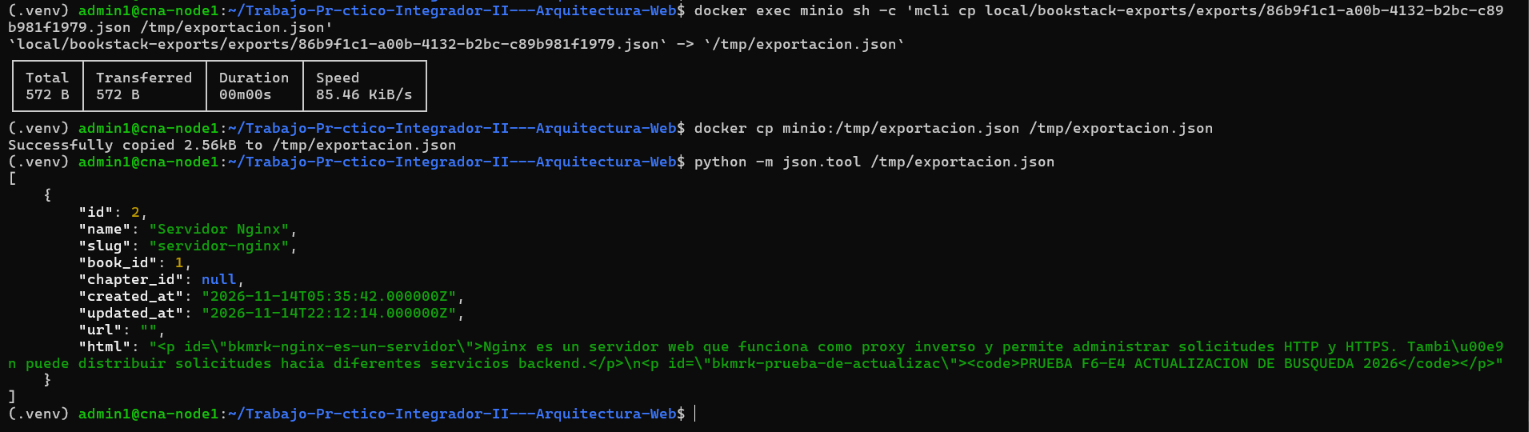
\includegraphics[width=0.9\linewidth,height=0.42\textheight,keepaspectratio]{F6-E6_04_contenido_json.png}
\caption{F6-E6: Ciclo completo de un job de exportación (parte 5)}
\label{fig:F6-E6-5}
\end{figure}
\begin{figure}[H]
\centering
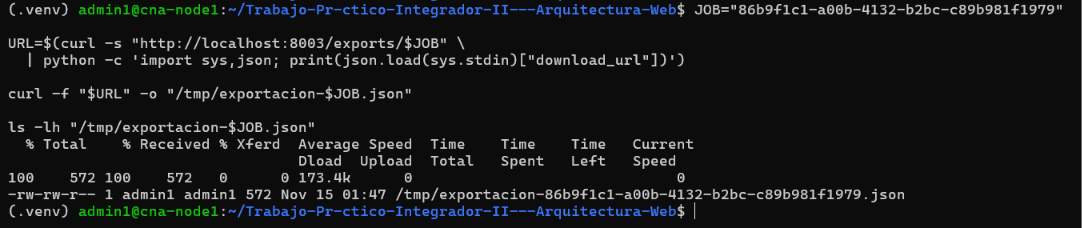
\includegraphics[width=0.9\linewidth,height=0.42\textheight,keepaspectratio]{F6-E6_05_descarga_presigned_url.png}
\caption{F6-E6: Ciclo completo de un job de exportación (parte 6)}
\label{fig:F6-E6-6}
\end{figure}
\subsubsection*{F6-E7 (P39) -- Objeto exportado en MinIO}
\begin{figure}[H]
\centering
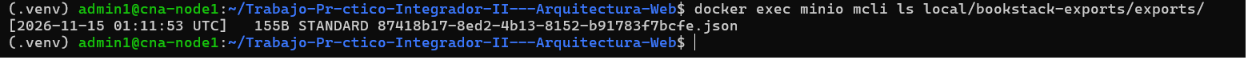
\includegraphics[width=0.9\linewidth,height=0.42\textheight,keepaspectratio]{F6-E7_01_objeto_almacenado_minio.png}
\caption{F6-E7: Objeto exportado en MinIO}
\label{fig:F6-E7-1}
\end{figure}
\subsubsection*{F6-E8 (P40) -- Subida y miniatura vía gateway}
\begin{figure}[H]
\centering
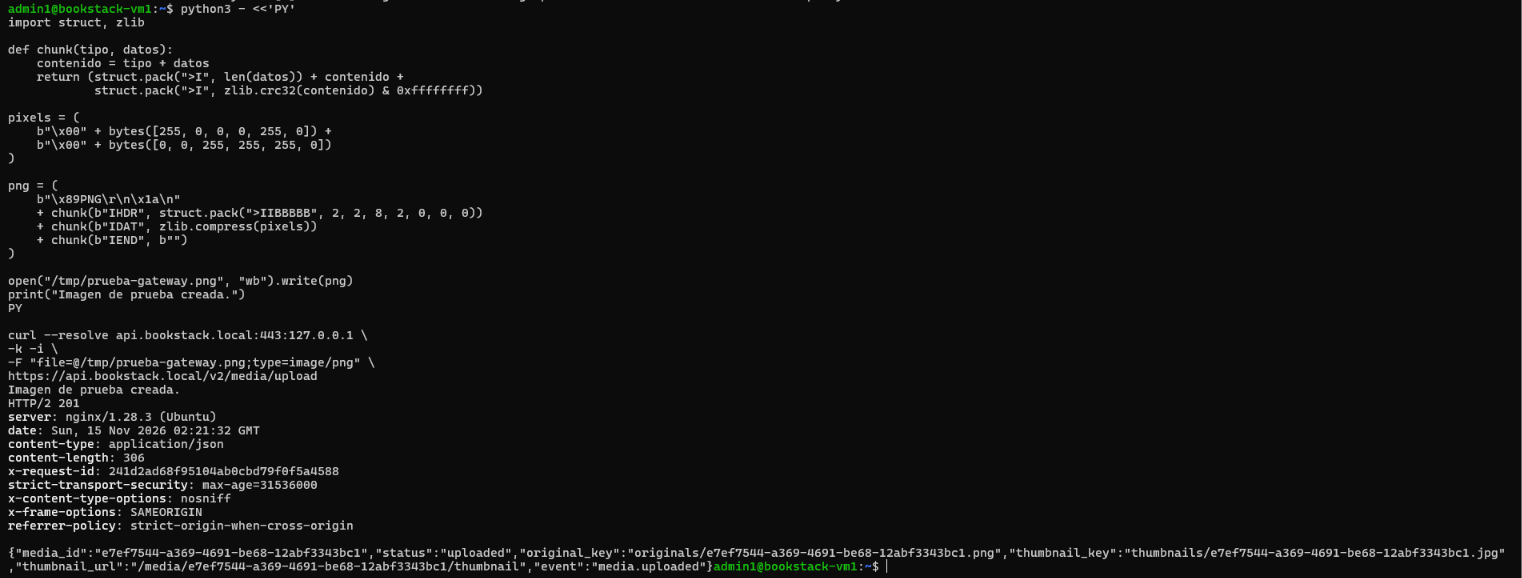
\includegraphics[width=0.9\linewidth,height=0.42\textheight,keepaspectratio]{F6-E8_01_subida_imagen_gateway.png}
\caption{F6-E8: Subida y miniatura vía gateway (parte 1)}
\label{fig:F6-E8-1}
\end{figure}
\begin{figure}[H]
\centering
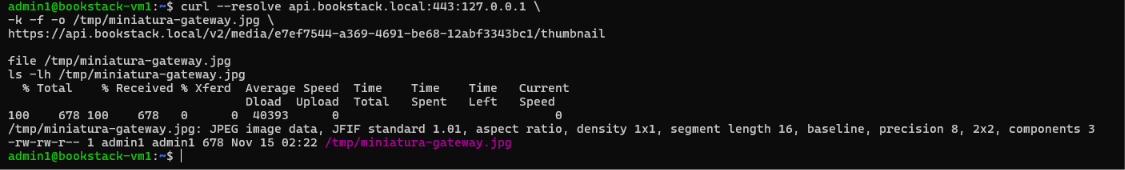
\includegraphics[width=0.9\linewidth,height=0.42\textheight,keepaspectratio]{F6-E8_02_miniatura_descargada_gateway.png}
\caption{F6-E8: Subida y miniatura vía gateway (parte 2)}
\label{fig:F6-E8-2}
\end{figure}
\begin{figure}[H]
\centering
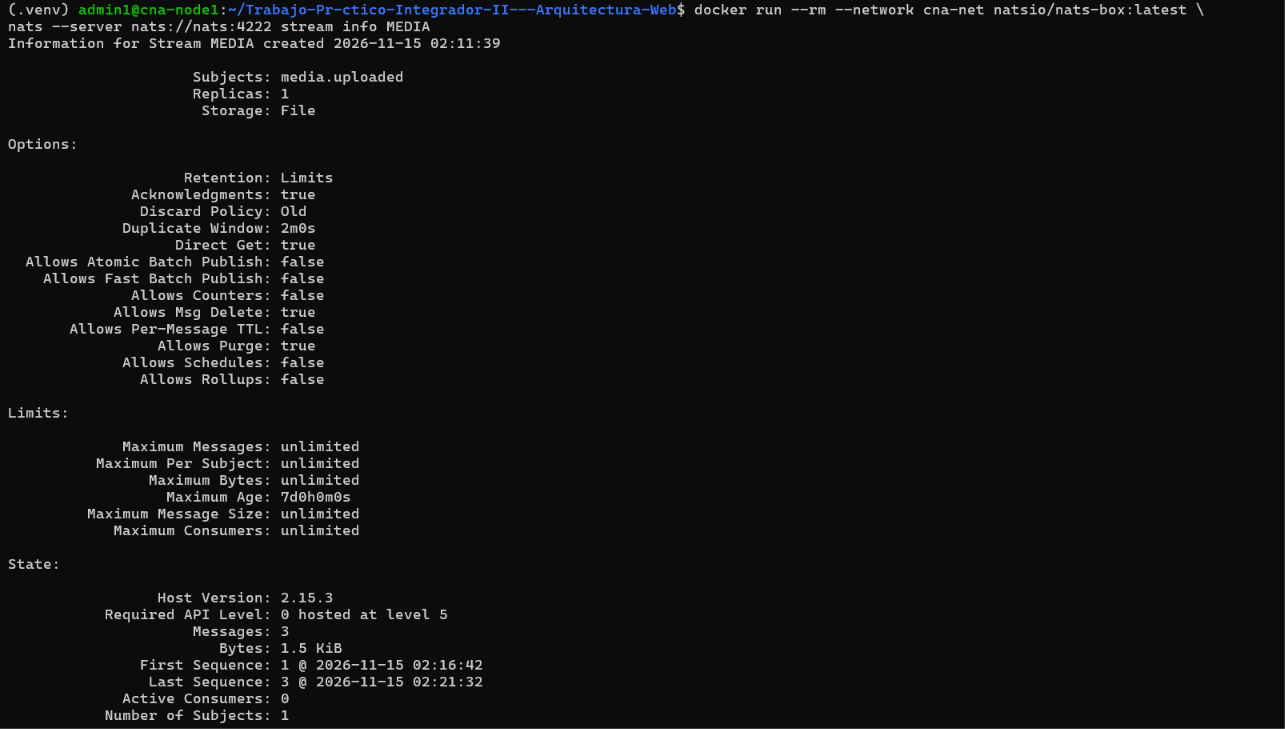
\includegraphics[width=0.9\linewidth,height=0.42\textheight,keepaspectratio]{F6-E8_03_evento_media_uploaded_nats.png}
\caption{F6-E8: Subida y miniatura vía gateway (parte 3)}
\label{fig:F6-E8-3}
\end{figure}
\subsubsection*{F6-E9 (P41) -- Etiquetas y tamaños de imágenes}
\begin{figure}[H]
\centering
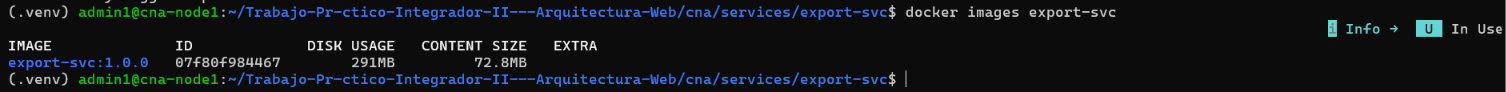
\includegraphics[width=0.9\linewidth,height=0.42\textheight,keepaspectratio]{F6-E9_01_imagen_export_svc.png}
\caption{F6-E9: Etiquetas y tamaños de imágenes}
\label{fig:F6-E9-1}
\end{figure}
\subsubsection*{F6-E10 (P42) -- docker inspect: usuario, límites, healthcheck}
\begin{figure}[H]
\centering
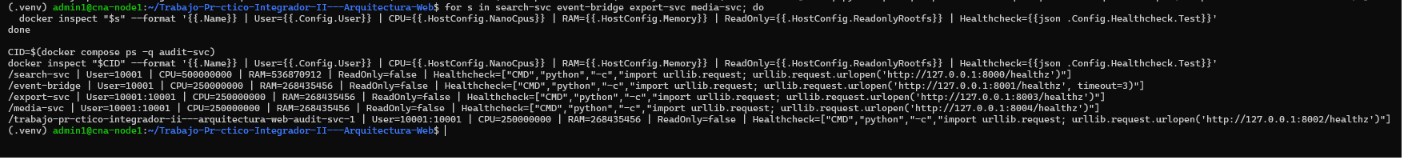
\includegraphics[width=0.9\linewidth,height=0.42\textheight,keepaspectratio]{F6-E10_01_inspeccion_contenedores.png}
\caption{F6-E10: docker inspect: usuario, límites, healthcheck}
\label{fig:F6-E10-1}
\end{figure}
\subsubsection*{F6-E11 (P43) -- Webhook configurado en BookStack}
\begin{figure}[H]
\centering
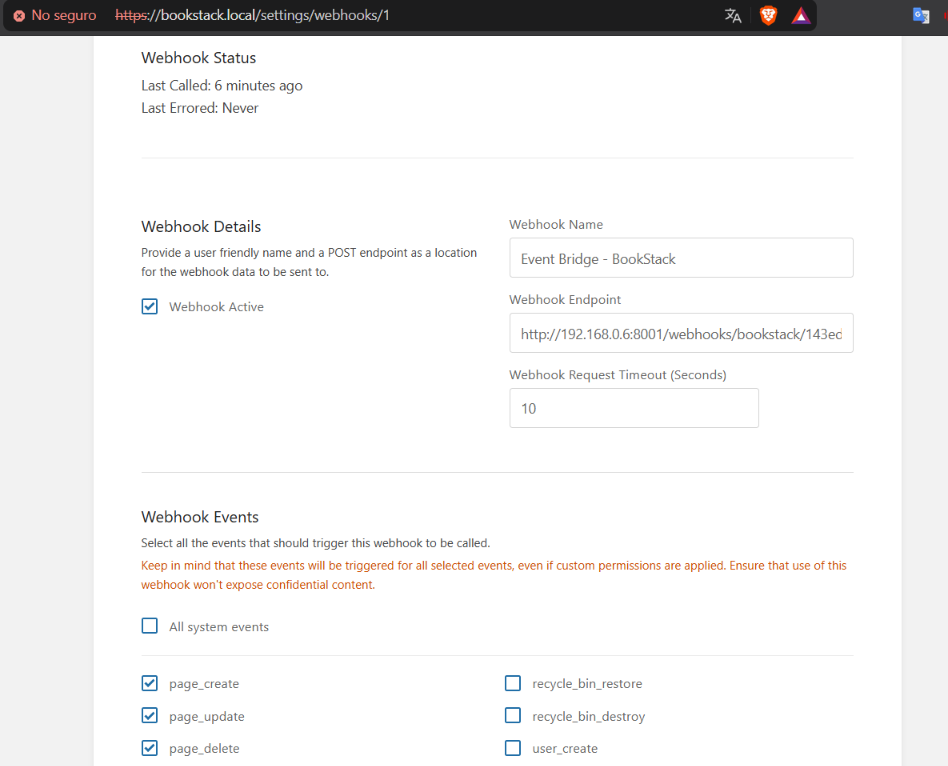
\includegraphics[width=0.9\linewidth,height=0.42\textheight,keepaspectratio]{F6-E11_webhook_bookstack.png}
\caption{F6-E11: Webhook configurado en BookStack}
\label{fig:F6-E11-1}
\end{figure}
\subsubsection*{F6-E12 (P44) -- Evento recibido en el broker}
\begin{figure}[H]
\centering
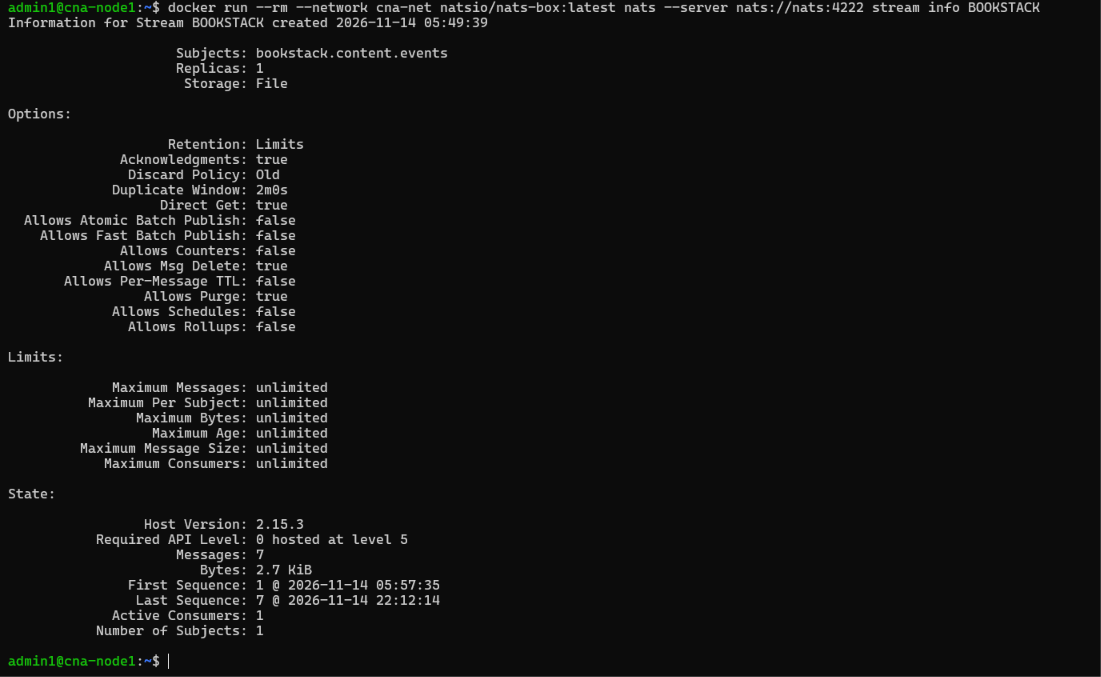
\includegraphics[width=0.9\linewidth,height=0.42\textheight,keepaspectratio]{F6-E12_01_stream_bookstack.png}
\caption{F6-E12: Evento recibido en el broker (parte 1)}
\label{fig:F6-E12-1}
\end{figure}
\begin{figure}[H]
\centering
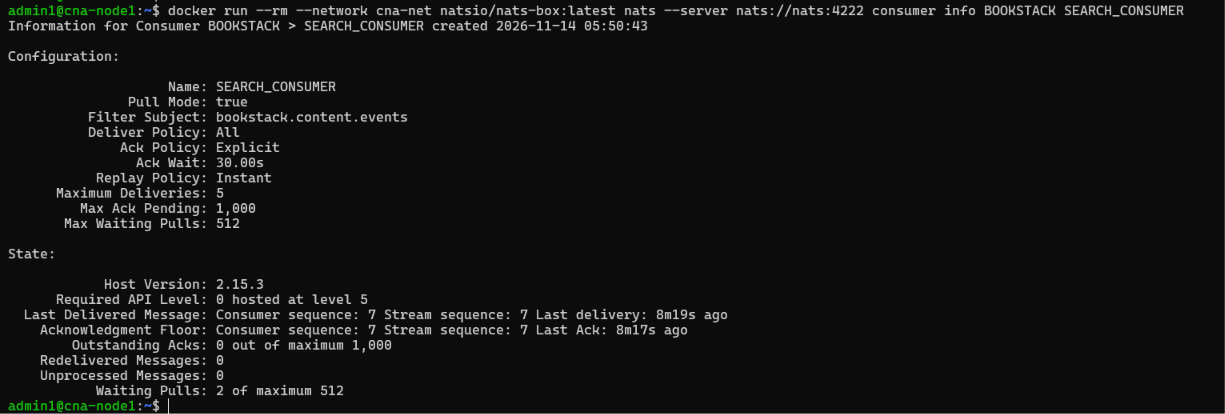
\includegraphics[width=0.9\linewidth,height=0.42\textheight,keepaspectratio]{F6-E12_02_consumer_search.png}
\caption{F6-E12: Evento recibido en el broker (parte 2)}
\label{fig:F6-E12-2}
\end{figure}
\subsubsection*{F6-E13 (P45) -- Mensaje enviado a la DLQ}
\begin{figure}[H]
\centering
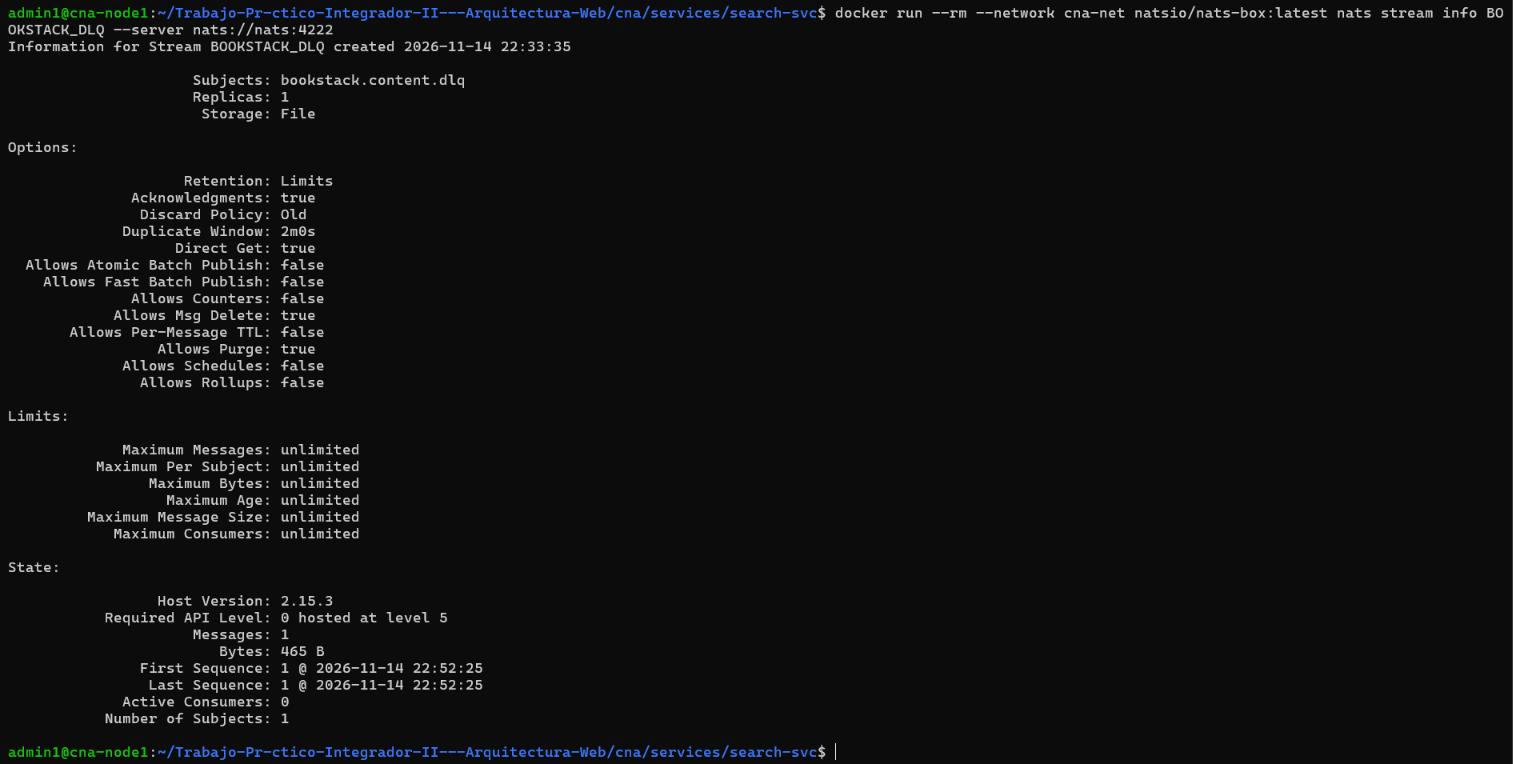
\includegraphics[width=0.9\linewidth,height=0.42\textheight,keepaspectratio]{F6-E13_01_mensaje_almacenado_DLQ.png}
\caption{F6-E13: Mensaje enviado a la DLQ (parte 1)}
\label{fig:F6-E13-1}
\end{figure}
\begin{figure}[H]
\centering
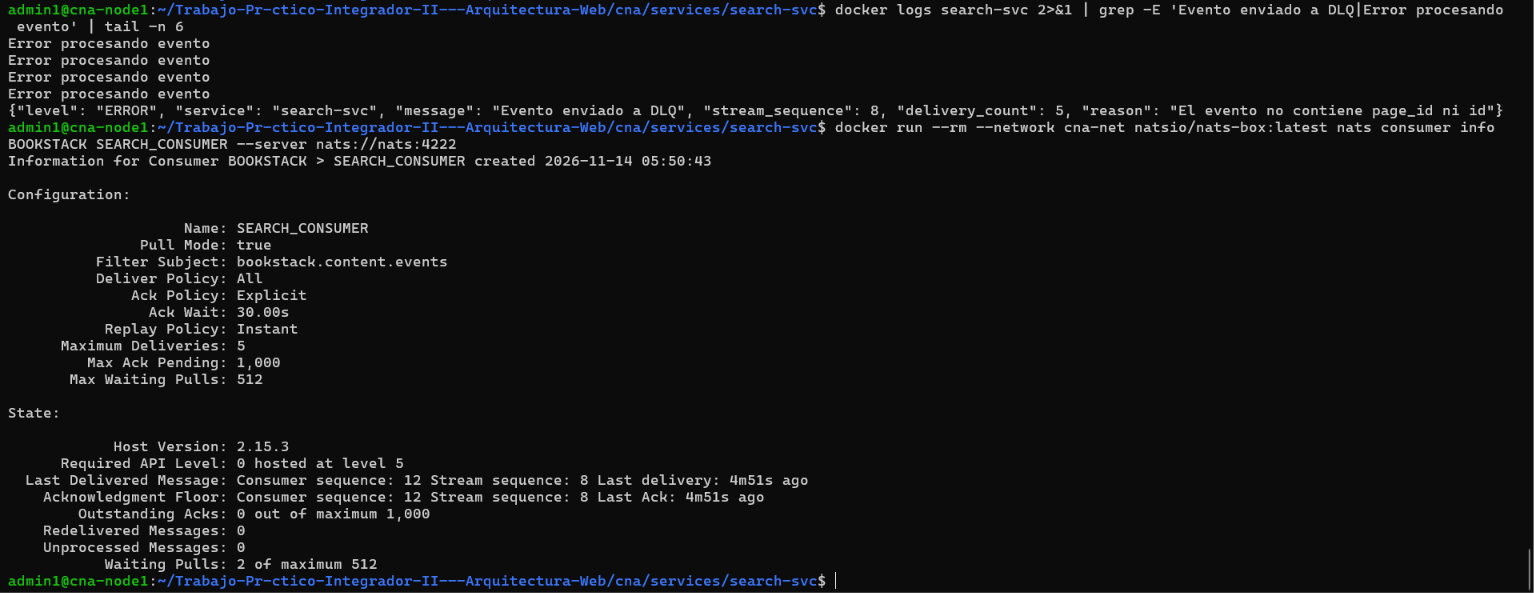
\includegraphics[width=0.9\linewidth,height=0.42\textheight,keepaspectratio]{F6-E13_02_quinto_intento_y_confirmacion.png}
\caption{F6-E13: Mensaje enviado a la DLQ (parte 2)}
\label{fig:F6-E13-2}
\end{figure}
\subsubsection*{F6-E14 (P46) -- nginx -t y server block del gateway}
\begin{figure}[H]
\centering
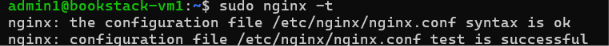
\includegraphics[width=0.9\linewidth,height=0.42\textheight,keepaspectratio]{F6-E14_01_nginx_test_correcto.png}
\caption{F6-E14: nginx -t y server block del gateway (parte 1)}
\label{fig:F6-E14-1}
\end{figure}
\begin{figure}[H]
\centering
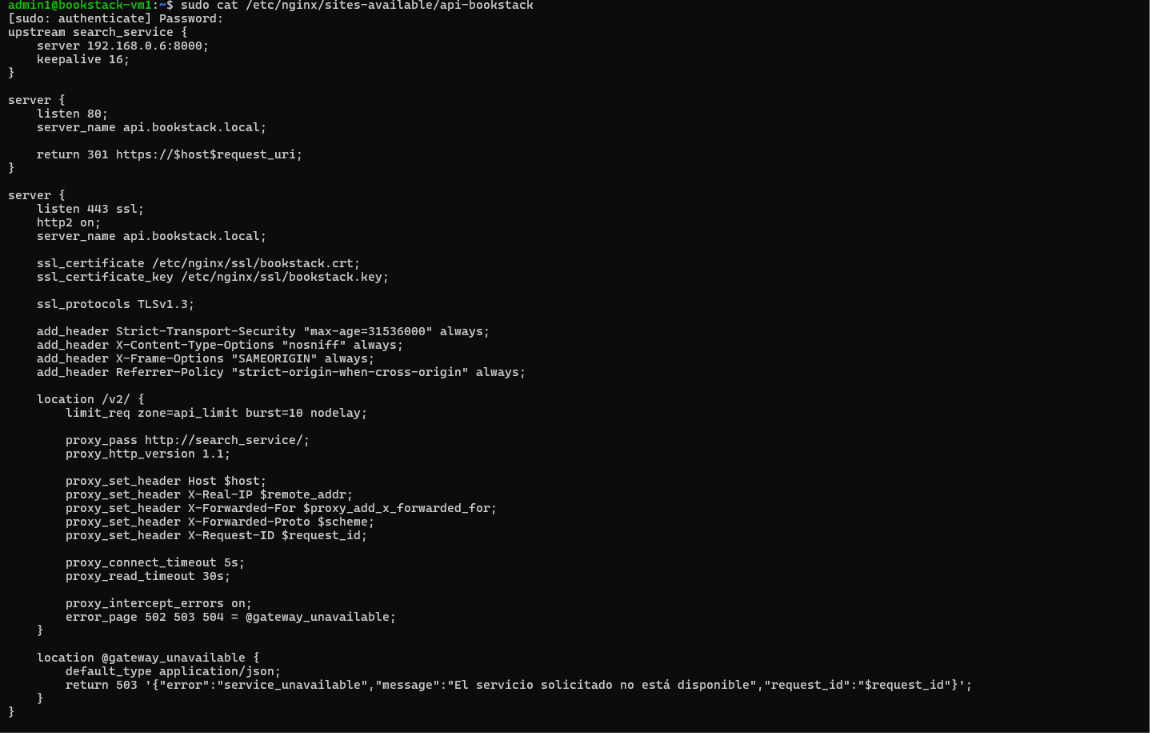
\includegraphics[width=0.9\linewidth,height=0.42\textheight,keepaspectratio]{F6-E14_02_server_block_gateway.png}
\caption{F6-E14: nginx -t y server block del gateway (parte 2)}
\label{fig:F6-E14-2}
\end{figure}
\begin{figure}[H]
\centering
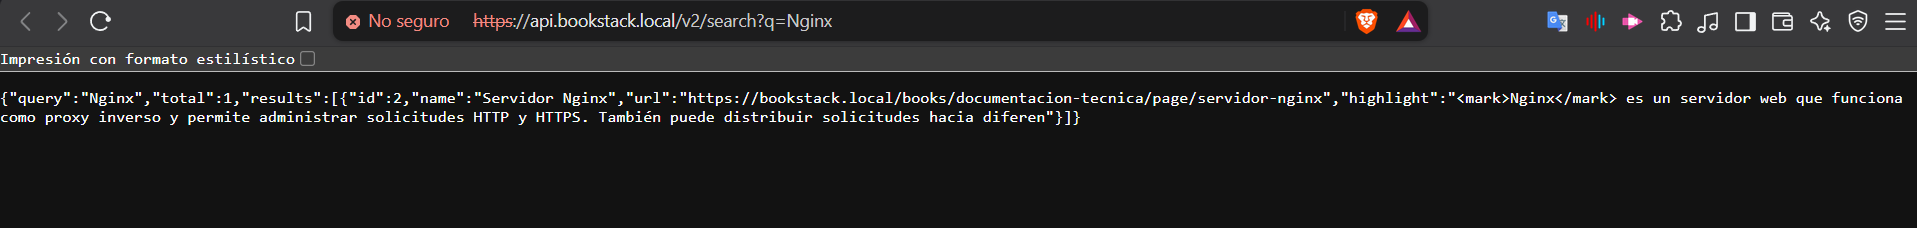
\includegraphics[width=0.9\linewidth,height=0.42\textheight,keepaspectratio]{F6-E14_03_gateway_busqueda_funcional.png}
\caption{F6-E14: nginx -t y server block del gateway (parte 3)}
\label{fig:F6-E14-3}
\end{figure}
\begin{figure}[H]
\centering
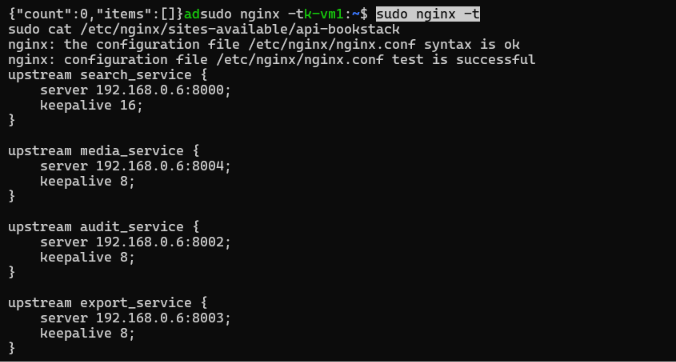
\includegraphics[width=0.9\linewidth,height=0.42\textheight,keepaspectratio]{F6-E14_04_gateway_cuatro_microservicios.png}
\caption{F6-E14: nginx -t y server block del gateway (parte 4)}
\label{fig:F6-E14-4}
\end{figure}
\subsubsection*{F6-E15 (P47) -- Respuesta 429 por rate limiting}
\begin{figure}[H]
\centering
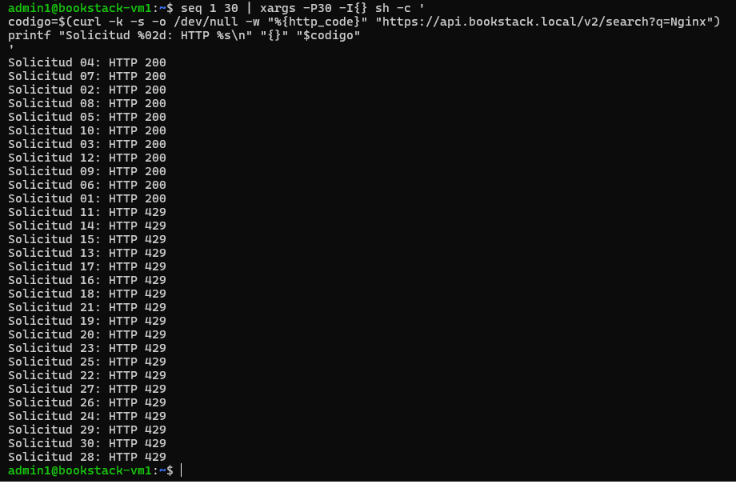
\includegraphics[width=0.9\linewidth,height=0.42\textheight,keepaspectratio]{F6-E15_01_rate_limiting_429.png}
\caption{F6-E15: Respuesta 429 por rate limiting}
\label{fig:F6-E15-1}
\end{figure}
\subsubsection*{F6-E16 (P48) -- Despliegue en un comando, servicios healthy}
\begin{figure}[H]
\centering
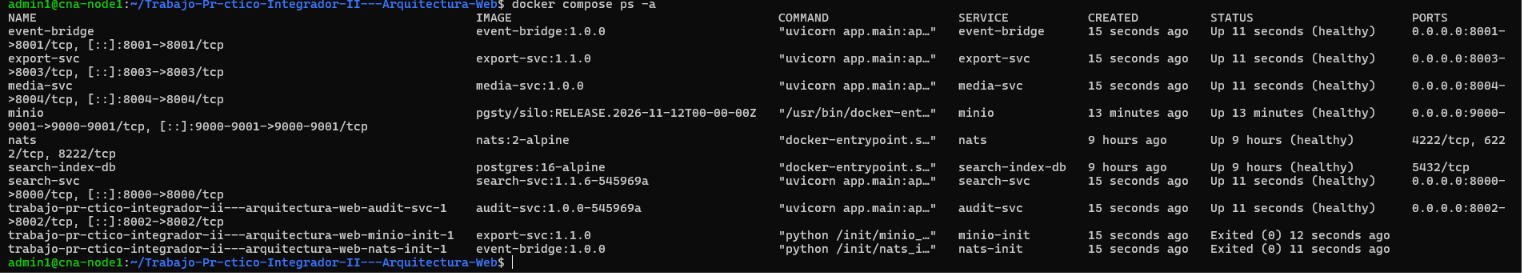
\includegraphics[width=0.9\linewidth,height=0.42\textheight,keepaspectratio]{F6-E16_01_despliegue_completo_healthy.png}
\caption{F6-E16: Despliegue en un comando, servicios healthy}
\label{fig:F6-E16-1}
\end{figure}

\newpage
%=====================================================================
\section{Fase 7: operación cloud native}
%=====================================================================
El procedimiento completo de cada experimento y medición está en \texttt{cna/docs/runbook\_fase7.md}. Cada script deja un log con marcas de tiempo en \texttt{cna/docs/evidencias/fase7/}, cuya primera línea muestra \texttt{usuario@host} para identificar el nodo.

\subsection{C1: resiliencia y experimentos de caos}
\begin{description}
  \item[X1 (F7-E1).] Caída de search-svc con \texttt{kill -9} sobre el proceso: el monolito sigue respondiendo 200, el gateway devuelve 503 JSON y el orquestador recrea el servicio; se mide el MTTR. Se usa \texttt{kill -9} y no \texttt{docker kill} porque, con Compose, \texttt{docker kill} cuenta como parada manual y \texttt{restart: unless-stopped} no reinicia el contenedor.
  \item[X2 (F7-E2).] audit-svc detenido 2 minutos mientras se editan 20 páginas: los eventos quedan en el stream durable y se procesan todos al volver (cero pérdida, CA-6).
  \item[X3 (F7-E3).] Se mata un export-worker con un job en \texttt{running}: el \emph{lease} en Redis vence y otro worker lo retoma hasta \texttt{done}.
  \item[X4 (F7-E4).] Apagado completo de VM-2: BookStack sigue operativo (CA-5) y el sistema converge solo al volver.
  \item[X5 (F7-E5).] 2 s de latencia hacia BookStack con \texttt{tc netem}: search-svc aplica timeout, reintentos con backoff y abre el interruptor de circuito; \texttt{/search} sigue respondiendo desde el índice local.
\end{description}

\subsection{C2: escalabilidad}
Pruebas de carga con k6 (monolito vs. \texttt{/v2/search}, 10 y 50 usuarios concurrentes) contra la línea base de la Fase 4 (F7-E6), escalado de export-worker de 1 a 3 réplicas midiendo jobs por minuto (F7-E7) y consumo de recursos por nodo con \texttt{docker stats} (F7-E8).

\subsection{C3: observabilidad}
Prometheus recolecta las métricas RED de los cinco servicios y la profundidad de las colas de JetStream; Grafana provisiona el tablero RED (F7-E9). Loki y Alloy agregan los logs JSON de todos los contenedores y del gateway, filtrables por \texttt{request\_id} (F7-E10). OpenTelemetry propaga el contexto de traza en las cabeceras de NATS, de modo que Jaeger muestra la edición completa: webhook, publicación, reindexación y auditoría (F7-E11). Las reglas de alerta (servicio caído, backlog de consumidor, circuito abierto) se disparan durante los experimentos (F7-E12).

\subsection{C4: seguridad}
Se escanearon las imágenes con Trivy 0.67.2 y se generó un SBOM CycloneDX con Syft 1.33.0 (F7-E13). \texttt{search-svc:2.0.0} no tiene vulnerabilidades CRITICAL y sus 47 HIGH corresponden a paquetes de Debian sin parche publicado. El token de la API de BookStack se rota sin reiniciar los servicios (F7-E14).

\begin{longtable}{>{\raggedright}p{0.8cm} >{\raggedright}p{4.2cm} >{\raggedright}p{1.5cm} >{\raggedright\arraybackslash}p{8cm}}
\caption{Registro de hallazgos de seguridad (amplía la sección 7.5 del TP I).}\\
\toprule ID & Hallazgo & Estado & Tratamiento \\ \midrule \endfirsthead
\toprule ID & Hallazgo & Estado & Tratamiento \\ \midrule \endhead
H-01 & Token del webhook visible en logs, métricas y trazas & Corregido & Plantilla de ruta, sin access log, redacción en las trazas. \\
H-02 & Pillow con 5 CVE CRITICAL en media-svc & Corregido & Pillow 13.0.0 y python-multipart 0.0.30. \\
H-03 & Starlette y zlib con HIGH en todas las imágenes & Corregido & FastAPI 0.163.1 + Starlette 1.3.1 y \texttt{apt-get upgrade}. \\
H-04 & 47 HIGH de Debian sin parche & Riesgo aceptado & UID 10001, \texttt{read\_only}, reescaneo en cada entrega. \\
H-05 & Rotar el token exigía recrear servicios & Corregido & Recarga en caliente del token (F7-E14). \\
H-06 & Alloy monta el socket de Docker & Riesgo aceptado & Montaje de solo lectura, sin puertos publicados. \\
H-07 & Puertos de Docker no filtrados por UFW & Corregido & Reglas en \texttt{DOCKER-USER} con \texttt{-i <interfaz>}. \\
H-08 & Etiquetas sin hash del commit & Corregido (Swarm) & Etiqueta \texttt{<versión>-<commit>}. \\
H-09 & API pública sin autenticación & Corregido & Middleware Bearer en los cuatro servicios. \\
\bottomrule
\end{longtable}

%=====================================================================
\section{Matriz consolidada de pruebas (P26 a P62)}
%=====================================================================
\begin{longtable}{|p{0.9cm}|p{1.3cm}|p{0.9cm}|p{5.6cm}|p{5.6cm}|}
\caption{Matriz de pruebas de las Fases 5 a 7 (continúa la Tabla 5 del TP I).}\\
\hline \textbf{Prueba} & \textbf{Evid.} & \textbf{Ítem} & \textbf{Descripción} & \textbf{Resultado} \\ \hline \endfirsthead
\hline \textbf{Prueba} & \textbf{Evid.} & \textbf{Ítem} & \textbf{Descripción} & \textbf{Resultado} \\ \hline \endhead
P26 & F5-E1 & A1 & Tablas por módulo vía information\_schema & Cumple: tablas agrupadas por módulo. \\ \hline
P27 & F5-E2 & A1 & Matriz de acoplamiento módulo × tabla & Cumple: matriz y relaciones polimórficas. \\ \hline
P28 & F5-E3 & A1 & Mapa de contextos (DDD) & Cumple. \\ \hline
P29 & F5-E4 & A3 & Contratos OpenAPI/AsyncAPI validados & Cumple: validación sin errores. \\ \hline
P30 & F5-E5 & A4 & Diagrama C4 nivel 1 (contexto) & Cumple. \\ \hline
P31 & F5-E6 & A4 & Diagrama C4 nivel 2 (contenedores) & Cumple. \\ \hline
P32 & F5-E7 & A4 & Diagramas de secuencia con caminos de error & Cumple: 3 secuencias. \\ \hline
P33 & F6-E1 & B1 & Nodos activos del motor Docker & Cumple. \\ \hline
P34 & F6-E2 & B1 & ufw status verbose de cada nodo & Cumple en VM-2 (firewall persistente, H-07). \\ \hline
P35 & F6-E3 & B1 & Certificado X.509 con doble SAN & Cumple. \\ \hline
P36 & F6-E4 & B2.1 & Búsqueda vía gateway antes/después de editar & Cumple: reindexación por evento. \\ \hline
P37 & F6-E5 & B2.2 & Idempotencia ante evento duplicado & Cumple: un solo registro. \\ \hline
P38 & F6-E6 & B2.3 & Ciclo completo de un job de exportación & Cumple: queued → done, URL prefirmada. \\ \hline
P39 & F6-E7 & B2.3 & Objeto exportado en MinIO & Cumple. \\ \hline
P40 & F6-E8 & B2.4 & Subida y miniatura vía gateway & Cumple: evento media.uploaded. \\ \hline
P41 & F6-E9 & B3 & Etiquetas y tamaños de imágenes & Cumple parcial: captura de export-svc. \\ \hline
P42 & F6-E10 & B3 & docker inspect: usuario, límites, healthcheck & Cumple. \\ \hline
P43 & F6-E11 & B4 & Webhook configurado en BookStack & Cumple. \\ \hline
P44 & F6-E12 & B4 & Evento recibido en el broker & Cumple: stream y consumidor durable. \\ \hline
P45 & F6-E13 & B4 & Mensaje enviado a la DLQ & Cumple: DLQ tras 5 intentos. \\ \hline
P46 & F6-E14 & B5 & nginx -t y server block del gateway & Cumple. \\ \hline
P47 & F6-E15 & B5 & Respuesta 429 por rate limiting & Cumple. \\ \hline
P48 & F6-E16 & B5 & Despliegue en un comando, servicios healthy & Cumple. \\ \hline
P49 & F7-E1 & C1 & X1: caída de S1 y MTTR & Ver log de x1-kill-search.sh. \\ \hline
P50 & F7-E2 & C1 & X2: cero pérdida de eventos en S2 & Ver log de x2-stop-audit.sh. \\ \hline
P51 & F7-E3 & C1 & X3: reintento de job tras caída de worker & Ver log de x3-kill-worker.sh. \\ \hline
P52 & F7-E4 & C1 & X4: apagado de VM-2 y convergencia & Ver log de x4-vm2-down.sh. \\ \hline
P53 & F7-E5 & C1 & X5: timeout, backoff e interruptor de circuito & Ver log de x5-bookstack-latency.sh. \\ \hline
P54 & F7-E6 & C2 & Resultados k6: monolito vs. S1 & Ver comparativa.md de run-k6.sh. \\ \hline
P55 & F7-E7 & C2 & Escalado de export-worker 1 → 3 & Ver F7-E7-export-tabla.md. \\ \hline
P56 & F7-E8 & C2 & Consumo de recursos por nodo & Ver CSV de capture-stats.sh. \\ \hline
P57 & F7-E9 & C3 & Tablero RED en Grafana & Tablero cna-red.json provisionado. \\ \hline
P58 & F7-E10 & C3 & Logs correlacionados por request\_id & Loki + Alloy, filtro por request\_id. \\ \hline
P59 & F7-E11 & C3 & Traza distribuida en Jaeger & OpenTelemetry con contexto en cabeceras NATS. \\ \hline
P60 & F7-E12 & C3 & Alerta disparada & Reglas en rules/alerts.yml. \\ \hline
P61 & F7-E13 & C4 & Informe Trivy y SBOM & search-svc:2.0.0: 0 CRITICAL, 47 HIGH sin parche (H-04); SBOM CycloneDX. \\ \hline
P62 & F7-E14 & C4 & Rotación del token de API & rotate-bookstack-token.sh, recarga en caliente (H-05). \\ \hline
\end{longtable}

\section{Conclusiones}
El monolito sigue funcionando sin cambios en su código mientras cuatro capacidades se extrajeron como servicios independientes, comunicados por eventos durables y expuestos por un gateway con TLS, límite de tasa y autenticación. La Fase 7 agregó la capacidad de observar el sistema, medir su recuperación ante fallos y gestionar sus vulnerabilidades y credenciales.

\end{document}
